\documentclass[UTF8]{ctexart}
\usepackage{amsmath}
\usepackage{amssymb}
\usepackage{graphicx}
\usepackage{geometry}
\usepackage{ctex}
\usepackage{amsmath}
\usepackage{amssymb}
\usepackage{xcolor}
\usepackage{geometry}
\usepackage{listings}
\usepackage{geometry}
\usepackage{marginnote}

\geometry{a4paper, margin=1in}

% Style for code blocks
\definecolor{codegreen}{rgb}{0,0.6,0}
\definecolor{codegray}{rgb}{0.5,0.5,0.5}
\definecolor{codepurple}{rgb}{0.58,0,0.82}
\definecolor{backcolour}{rgb}{0.95,0.95,0.95}

\lstdefinestyle{mystyle}{
    backgroundcolor=\color{backcolour},   
    commentstyle=\color{codegreen},
    keywordstyle=\color{magenta},
    numberstyle=\tiny\color{codegray},
    stringstyle=\color{codepurple},
    basicstyle=\ttfamily\footnotesize,
    breakatwhitespace=false,         
    breaklines=true,                 
    captionpos=b,                    
    keepspaces=true,                 
    numbers=left,                    
    numbersep=5pt,                  
    showspaces=false,                
    showstringspaces=false,
    showtabs=false,                  
    tabsize=2
}
\lstset{style=mystyle}
\geometry{a4paper, margin=1in}

\title{QTA2025暑期求职笔试训练营-week2}
\author{欧岱松}
\date{\today{}}

\begin{document}

\maketitle

\section*{笔试题目}

\subsection*{1. 随机数}
小U有一个质地不均匀的硬币, 已知这枚硬币正面朝上的概率$p$不是0或0.5, 但不知道确切的概率, 可以只用这枚硬币帮小U生成100个0-15之间均匀分布的随机整数吗? 小U是个追求严谨的小朋友, 如果可以, 需要聪明的你证明这种策略下生成的随机数的分布严格服从上述要求; 如果不可以, 也请给出证明。

这个问题的核心在于如何利用有偏的随机源来构建概率均等的随机数,我们考虑如下策略,将硬币连续抛掷两次 :
\begin{itemize}
    \item 如果结果是 正-反 (HT),我们就将其记为 0。

    \item 如果结果是 反-正 (TH),我们就将其记为 1。
    
    \item 如果结果是 正-正 (HH) 或 反-反 (TT),我们就舍弃这次结果,重新抛掷两次。    
    
\end{itemize}

\textbf{第一步:验证该策略确实可以生成我们要求的随机数}

设硬币正面朝上的概率为 $p$,反面朝上的概率为 $1-p$(其中 $p \neq 0, 0.5, 1$)。

计算各种情况的概率:
\begin{align}
P(HT) &= p \cdot (1-p) \\
P(TH) &= (1-p) \cdot p = p \cdot (1-p) \\
P(HH) &= p^2 \\
P(TT) &= (1-p)^2
\end{align}

注意到$P(HT) = P(TH) = p(1-p)$

在条件概率下:
\begin{align}
P(\text{输出0} | \text{不拒绝}) &= \frac{P(HT)}{P(HT) + P(TH)} =
\frac{p(1-p)}{2p(1-p)} = \frac{1}{2} \\
P(\text{输出1} | \text{不拒绝}) &= \frac{P(TH)}{P(HT) + P(TH)} =
\frac{p(1-p)}{2p(1-p)} = \frac{1}{2}
\end{align}

因此,每次生成的随机数都是公平的,即 $P(\text{输出0}) = P(\text{输出1}) =
\frac{1}{2}$。

\textbf{第二步:生成0-15的均匀分布}

考虑到是生成16个数,我们可以二进制来处理,具体来说:
\begin{enumerate}
    \item 使用上述方法生成4个概率均等的随机数 $b_3b_2b_1b_0$
    \item 将这上面的随机数转换为整数:$n = 8b_3 + 4b_2 + 2b_1 + b_0$
    \item 由于 $n \in \{0,1,2,\ldots,15\}$,直接输出 $n$
\end{enumerate}


由于每次生成的单个随机数都是独立且公平的($P(b_i = 0) = P(b_i = 1) = \frac{1}{2}$),所以:

$$P(n = k) = P(b_3b_2b_1b_0 \text{的二进制表示为} k) = \left(\frac{1}{2}\right)^4 =
\frac{1}{16}$$

对于所有 $k \in \{0,1,2,\ldots,15\}$ 都成立。

\textbf{第三步:生成100个随机数:}

重复上述过程100次,每次生成一个0-15之间的随机整数。由于每次生成都是独立的,且每个整
数的概率都是 $\frac{1}{16}$,所以生成的100个数严格服从0-15的均匀分布。

\subsection*{2. 剪纸转圈圈}

(1) 小U在做剪纸小游戏, 他先剪了一大一小两个圆, 如图2所示, 其中圆A的半径为1, 圆B的半径为5。现在让小圆A绕着大圆B滚动旋转, 请问小圆A旋转多少圈后其圆心将再次到达起点?

\textbf{我们在这里默认,小圆带动大圆的滚动旋转会使得大圆发生相应的滚动(否则,这个问题是平凡的,即5圈),进一步可以将小圆的旋转进行分解}
\begin{itemize}
    \item \textbf{小圆滚动产生的自转}:这部分等于两圆周长之比,即 $C_B / C_A = (2\pi R)/(2\pi r) = R/r = 5/1 = 5$ 圈。 
    \item \textbf{公转产生的自转}:小圆A的圆心绕大圆B的圆心完成了一整个圆周运动,这个公转本身会带来额外的1圈自转。
\end{itemize}
总圈数 = 滚动自转 + 公转自转 = $5 + 1 = 6$ 圈。

(2)小U又剪了一个边长为1的小正方形C, 现在让小正方形C在大圆B的圆周上移动一周 (保持正方形始终直立, 如图3), 请聪明的你帮小U算一算: 小正方形C平移一周所覆盖区域的面积是多少?

如图3所示,我们可以将正方形四个顶点,分别沿着四分之一圆周移动,并形成一个圆弧的平移,接着正方形在通过平移进入下一个圆周周期。为了简便计算,我们考虑将其补成一个12*12的正方形,再减去四周的圆弧和内部圆形即可。
$$
\begin{align}
    A &= 12^2 - (10^2-25\times \pi) -  25\tiems \pi\\
    &= 44 \\
\end{align}
$$
\begin{figure}[h!]
    \centering
    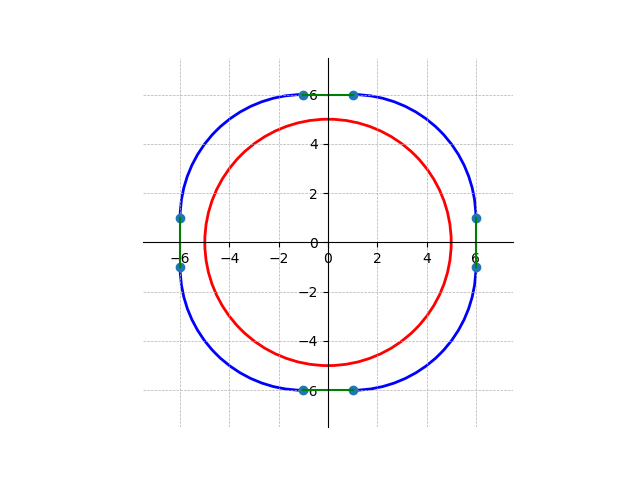
\includegraphics[width=0.8\linewidth]{coordinate_plane.png}
    \caption{物理情景示意图}
    \label{fig:fig3}
\end{figure}


\begin{figure}[h!]
    \centering
    \begin{minipage}{0.45\textwidth}
        \centering
        % The user needs to provide the image file 'figure1.png'
        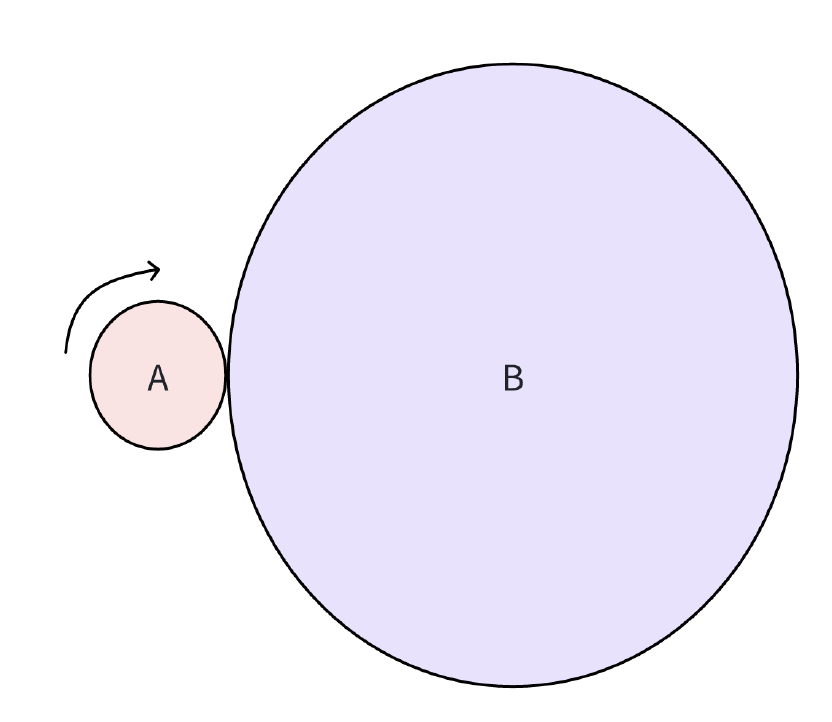
\includegraphics[width=0.8\linewidth]{Figure1.png} 
        \caption{小圆A绕大圆B滚动}
        \label{fig:fig1}
    \end{minipage}\hfill
    \begin{minipage}{0.45\textwidth}
        \centering
        % The user needs to provide the image file 'figure2.png'
        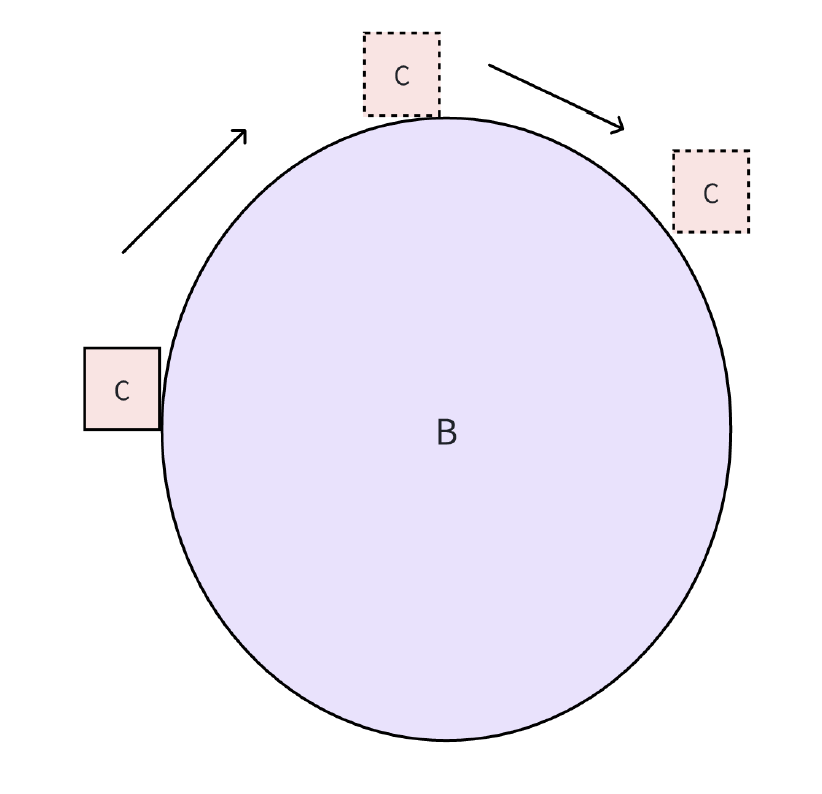
\includegraphics[width=0.8\linewidth]{Figure2.png}
        \caption{正方形C沿大圆B移动}
        \label{fig:fig2}
    \end{minipage}
\end{figure}


\subsection*{3. 正态分布}
概率论和微积分是一个quant需要熟练掌握的基础知识, 小U正在温习正态分布的相关内容。设 $\varphi(y)$ 和 $\Phi(y)$ 分别为标准正态分布的密度和分布函数, 求:

$$\int_{-\infty}^{+\infty}{\left(y+\frac{1}{\sqrt{\pi}}\right)^{2}(1-\Phi(y))\varphi
  (y)dy}$$
令要求解的积分为I,我们将采用对称性和分部积分法来解决。:
$$ I = \int_{-\infty}^{+\infty}{\left(y+\frac{1}{\sqrt{\pi}}\right)^{2}(1-\Phi(y))\varphi(y)dy} $$

\subsection*{1. 对称性换元}
我们利用标准正态分布的两个关键性质:密度函数 $\varphi(y)$ 是一个偶函数以及分布函数满足 $\Phi(-y) = 1 - \Phi(y)$

在积分 $I$ 中,令 $z = -y$,则 $y = -z$ ,得到:
$$ I = \int_{-\infty}^{+\infty}{\left(z-\frac{1}{\sqrt{\pi}}\right)^{2}(1-(1-\Phi(z)))\varphi(z)dz} $$
将变量 $z$ 换回 $y$,我们得到一个与原式等价的积分表达式:
$$ I = \int_{-\infty}^{+\infty}{\left(y-\frac{1}{\sqrt{\pi}}\right)^{2}\Phi(y)\varphi(y)dy} $$

\subsection*{2. 求解}
将两个等价的 $I$ 表达式相加,得到 $2I$:
$$ 2I = \int_{-\infty}^{+\infty} \left[ \left(y+\frac{1}{\sqrt{\pi}}\right)^{2}(1-\Phi(y)) + \left(y-\frac{1}{\sqrt{\pi}}\right)^{2}\Phi(y) \right] \varphi(y)dy $$
化简表达式得到:
$$ 2I = \int_{-\infty}^{+\infty} \left[ y^2 + \frac{1}{\pi} + \frac{2y}{\sqrt{\pi}}(1-2\Phi(y)) \right] \varphi(y)dy $$
现在,我们将积分拆分为三个部分:
$$ 2I = \int_{-\infty}^{+\infty} y^2 \varphi(y)dy + \frac{1}{\pi}\int_{-\infty}^{+\infty}\varphi(y)dy + \frac{2}{\sqrt{\pi}}\int_{-\infty}^{+\infty} y(1-2\Phi(y))\varphi(y)dy $$

\subsection*{3. 计算各部分积分}
\begin{itemize}
    \item \textbf{第一部分}: $\int_{-\infty}^{+\infty} y^2 \varphi(y)dy$ 是标准正态分布的二阶矩,等于其方差,即 \textbf{1}。
    \item \textbf{第二部分}: $\frac{1}{\pi}\int_{-\infty}^{+\infty}\varphi(y)dy$。根据概率密度函数的定义,$\int_{-\infty}^{+\infty}\varphi(y)dy=1$。所以,该项等于 \textbf{$\frac{1}{\pi}$}。
    \item \textbf{第三部分}: $\frac{2}{\sqrt{\pi}} \left[ \int y\varphi(y)dy - 2\int y\Phi(y)\varphi(y)dy \right]$
        \begin{itemize}
            \item 其中 $\int_{-\infty}^{+\infty} y\varphi(y)dy$ 是标准正态分布的均值,等于 0。
            \item 对于 $\int_{-\infty}^{+\infty} y\Phi(y)\varphi(y)dy$,通过分部积分可得其值为 $\frac{1}{2\sqrt{\pi}}$,具体计算过程见附录。
    
            \item 因此,第三部分的值为:$\frac{2}{\sqrt{\pi}} \left[ 0 - 2 \left( \frac{1}{2\sqrt{\pi}} \right) \right] = -\frac{2}{\pi}$。
        \end{itemize}
\end{itemize}

\subsection*{4. 汇总结果}
将三部分的结果代入 $2I$ 的表达式:
$$ 2I = 1 + \frac{1}{\pi} - \frac{2}{\pi} = 1 - \frac{1}{\pi} $$
最终,求解 $I$:
$$ I = \frac{1}{2} - \frac{1}{2\pi} $$

\subsection*{4. 打家劫舍}
小U在复习完数学后觉得coding也不能落下, 请聪明的你帮他设计一个时间复杂度尽可能小的算法, 求一个整数数组S中不含相邻元素的子序列的最大和。

我们考虑动态规划的方法来解决当前问题,可以取得理论最优的时间复杂度O(n)和空间复杂度O(1)。具体来说,我们从第一数组元素遍历每一个元素,
每一次比较获取之前的元素和获取当前元素的数组和哪一个更大。
\begin{lstlisting}[language=Python, caption=O(1) 空间复杂度 和 O(n) 时间复杂度的解法]
    def rob_optimized(S):
        """
        计算不含相邻元素的子序列的最大和
        param S: 一个整数数组
        return: 不含相邻元素的子序列的最大和
        """
        n = len(S)
        if n == 0:
            return 0
        
        # prev_max: 相当于 dp[i-2]
        # curr_max: 相当于 dp[i-1]
        prev_max = 0
        curr_max = 0
    
        for amount in S:
            # temp 用来临时存储 curr_max (即旧的 dp[i-1])
            temp = curr_max
            # 新的 curr_max (即 dp[i]) 是获取前一个元素的最大值(curr_max)与获得当前元素(amount + prev_max)的较大值
            curr_max = max(curr_max, amount + prev_max)
            # 更新 prev_max 为旧的 curr_max,为下一次迭代做准备
            prev_max = temp
    
        return curr_max
    # --- 示例数组 ---
    example_S = [2, 7, 9, 3, 1]

    # --- 调用函数并打印结果 ---
    max_sum = rob_optimized(example_S)
    print(f"对于示例数组 S = {example_S}")
    # 对于示例数组 S = [2, 7, 9, 3, 1]
    print(f"不含相邻元素的最大和为: {max_sum}") 
    # 不含相邻元素的最大和为: 12
\end{lstlisting}

\subsection*{5. Linear Regression Model}
Xiao U is learning English and regression analysis. Please help him solve the following problem:
Suppose we have a simple linear regression model,
$$ y_{j}=\beta_{0}+\beta_{1}x_{j}+\epsilon_{j}, \quad j=1,2,...,n $$
But the $x_{j}$ are independently $N(\mu_{x},\sigma_{x}^{2})$. We assume further that $\epsilon_{j}\sim N(0,\sigma_{e}^{2})$, independently of the $x_{j}$'s.
Suppose further that $x_{j}$ is in fact measured with error, so the observations are $(y_{j},w_{j})$, where
$$ w_{j}=x_{j}+u_{j}, \quad u_{j}\sim N(0,\sigma_{u}^{2}) $$
and $u$ is independent of both $x$ and $\epsilon$.
Now, please show that $E(y_{j}|w_{j})=\alpha_{0}+\alpha_{1}w_{j}$, and give expressions for $\alpha_{0}$ and $\alpha_{1}$ as functions of known constants.

因为$E(y_{j}|w_{j})=E(\beta_{0}+\beta_{1}x_{j}+\epsilon_{j}|w_{j})=\beta_{0}+E(\beta_{1}x_{j}+\epsilon_{j}|w_{j})=\beta_{0}+\beta_{1}E(x_{j}|w_{j})+E(\epsilon_{j}|w_{j})$
又因为$\epsilon_{j}$与$w_{j}$独立,所以$E(\epsilon_{j}|w_{j})=E(\epsilon_{j})=0$

对于$E(x_{j}|w_{j})$,我们可以应用附录中证明的正态分布条件期望公式。在本题中,$x_j$和$w_j$构成二元正态随机变量,其中:
\begin{itemize}
    \item $E(x_j) = \mu_x$
    \item $Var(x_j) = \sigma_x^2$
    \item $E(w_j) = E(x_j + u_j) = \mu_x + 0 = \mu_x$
    \item $Var(w_j) = Var(x_j + u_j) = \sigma_x^2 + \sigma_u^2$
    \item $Cov(x_j, w_j) = Cov(x_j, x_j + u_j) = Cov(x_j, x_j) + Cov(x_j, u_j) = \sigma_x^2 + 0 = \sigma_x^2$
\end{itemize}

根据附录中的条件期望公式:
$$E(X|Y=y) = E(X) + \frac{Cov(X,Y)}{Var(Y)}(y - E(Y))$$

代入我们的参数,整理得到:
$$
E(x_{j}|w_{j}) = \mu_{x} + \frac{\sigma_{x}^{2}}{\sigma_{x}^{2} + \sigma_{u}^{2}}(w_{j} - \mu_{x})
$$

$$E(y_{j}|w_{j}) = \beta_{0} + \beta_{1}\left[\mu_{x} + \frac{\sigma_{x}^{2}}{\sigma_{x}^{2} + \sigma_{u}^{2}}(w_{j} - \mu_{x})\right]$$


$$E(y_{j}|w_{j}) = \beta_{0} + \beta_{1}\mu_{x}\left(1-\frac{\sigma_{x}^{2}}{\sigma_{x}^{2} + \sigma_{u}^{2}}\right) + \beta_{1}\frac{\sigma_{x}^{2}}{\sigma_{x}^{2} + \sigma_{u}^{2}}w_{j}$$

令$\alpha_{0} = \beta_{0} + \beta_{1}\mu_{x}\left(1-\frac{\sigma_{x}^{2}}{\sigma_{x}^{2} + \sigma_{u}^{2}}\right)$,$\alpha_{1} = \beta_{1}\frac{\sigma_{x}^{2}}{\sigma_{x}^{2} + \sigma_{u}^{2}}$

则:
$$E(y_{j}|w_{j}) = \alpha_{0} + \alpha_{1}w_{j}$$
证明完毕。
\subsection*{6. 共半球问题}
\subsubsection*{(1)}
小U发现了一道经典的量化题: 圆上随机取N个点, 它们在同一个半圆内的概率有多大?

让我们先任意选择一个点,比如 \(P_1\),以 $P_1$ 为起点,顺时针画出一个半圆。我们称这个半圆为 $H_1$。要让所有其他 $N-1$ 个点都落在这个特定的半圆 $H_1$ 内,概率是多少?
\begin{itemize}
    \item 对于任何一个随机点 $P_i$ ($i \neq 1$),它落在 $H_1$ 内的概率是 $\frac{1}{2}$。
    \item 因为这 $N-1$ 个点的选择是相互独立的,所以它们全部落在 $H_1$ 内的概率是 $(\frac{1}{2})^{N-1}$。
\end{itemize}
并计这个事件为事件$A_i$,
\begin{itemize}
    \item $A_1$: 所有点都落在以 $P_1$ 为起点的顺时针半圆内。
    \item $A_2$: 所有点都落在以 $P_2$ 为起点的顺时针半圆内。
    \item \dots
    \item $A_N$: 所有点都落在以 $P_N$ 为起点的顺时针半圆内。
\end{itemize}
注意到,这N个事件的互斥的,且根据对称性,其概率相同均为$(\frac{1}{2})^{N-1}$。
\subsubsection*{(2)}
求知欲很强的小U继续探索, 假如问题变成3维球体呢? 即在球面上随机取N个点, 它们在同一个半球内的概率有多大?

事件是“所有N个点都落在某一个半球内”,同样,我们先任意选择一个点 $P_1$。这个点 $P_1$ 可以被看作是某个半球的“极点”。这个半球 $H_1$ 就是由过球心且垂直于 $\vec{OP_1}$ 向量的平面所定义的、$P_1$ 所在的那一半球面。
要让所有其他 $N-1$ 个点都落在这个特定的半球 $H_1$ 内,概率为$(\frac{1}{2})^{N-1}$。我们同样定义 $N$ 个事件 $A_i$:所有其他 $N-1$ 个点都落在以 $P_i$ 为“极点”的那个半球内。正如在二维情况中一样,这些事件也是相互排斥的。
$$ P(\text{所有点在同一个半球内}) = \sum_{i=1}^{N} P(A_i) = N \times \left(\frac{1}{2}\right)^{N-1} $$
\subsubsection*{(3) 【拓展思考题】}
在n维空间的球面上随机取N个点, 它们在同一个半球内的概率有多大?

类似的,维度的增加并没有改变问题的实质。在 $n$ 维空间中,一个“超半球”(hyper-hemisphere)是由一个通过球心的 $(n-1)$ 维超平面(hyperplane)将 $(n-1)$-球面切割成两半而得到的。
。因此,一个随机点落在指定超半球内的概率永远是 $\frac{1}{2}$。类似的事件$A_i$也是相互排斥的,且根据对称性,其概率相同均为$(\frac{1}{2})^{N-1}$。
$$ P(\text{所有点在同一个超半球内}) = \sum_{i=1}^{N} P(A_i) = N \times \left(\frac{1}{2}\right)^{N-1} $$
\subsection*{7. Pattern Problem}
小U在学习stochastic process, 他手里有一个不均匀的硬币, 每次掷到正面(H)的概率为p, 掷到反面(T)的概率为q, $p+q=1$, 请问首次掷到以下pattern的期望投掷次数为多少?
\begin{enumerate}
    \item HHHHHHTTTTTT
    \item HHHHHHHHHHHH
    \item HTHTHTTHTHT
\end{enumerate}

\subsubsection*{7.1 鞅停时定理求解}
假设我们有一枚不均匀的硬币,每次投掷得到正面(H)的概率为 $p$,得到反面(T)的概率为 $q$,其中 $p+q=1$。对于一个给定的、由 H 和 T 组成的模式 $S = s_1s_2...s_L$,我们的目标是计算首次观察到该模式所需的期望投掷次数,记为 $E$。

为了应用鞅理论,我们构造一个如下的假想公平赌局:
\begin{enumerate}
    \item \textbf{赌徒入场}:在每次投掷 $n=1, 2,  \dots$ 开始之前,都有一位新的赌徒 $C_n$ 加入赌局,并下注 1 元。
    \item \textbf{押注策略}:所有赌徒都采用相同的策略。赌徒 $C_n$ 在他入场时(即第 $n$ 次投掷),押注该次投掷结果为模式的第一个字符 $s_1$。如果他赢了,他将所有赢得的钱押在下一次(第 $n+1$ 次)投掷的结果是 $s_2$ 上,以此类推。只要输一次,他就失去所有钱并出局。
    \item \textbf{公平赔率}:为了使赌局对赌场和赌徒双方都公平,对于一次成功的押注,其赔付规则是:若押注的事件发生概率为 $P_e$,则 $1$ 元的赌注在成功后会变为 $1/P_e$ 元。
\end{enumerate}
在这个设定下,任何一次押注的期望净收益都为零,因此整个系统是公平的。


\textbf{7.1.1 构造鞅过程:}

令 $\mathcal{W}_n$ 表示在第 $n$ 次投掷结束后,赌场的累计净收益。这个随机过程 $\{\mathcal{W}_n\}_{n \ge 0}$ 是一个鞅(Martingale),因为它满足鞅性质:
$$ E[\mathcal{W}_{n+1} | \mathcal{F}_n] = \mathcal{W}_n $$
其中 $\mathcal{F}_n$ 代表直到时间 $n$ 的所有历史信息。由于赌局是公平的,赌场的期望收益在任何时刻都应保持不变。初始时 $\mathcal{W}_0 = 0$,故 $E[\mathcal{W}_n] = 0$ 对所有 $n$ 成立。

\textbf{7.1.2 应用鞅停时定理进行求解:}

我们定义一个停时 $\tau$ 为模式 $S$ 首次出现的时刻。即:
$$ \tau = \min\{ n \ge L : X_{n-L+1} \dots X_n = S \} $$
其中 $X_k$ 是第 $k$ 次投掷的结果。
根据鞅停时定理,在满足一定条件下(本问题的构造满足),鞅过程在停时的期望值等于其初始值:
$$ E[\mathcal{W}_\tau] = E[\mathcal{W}_0] = 0 $$
这个等式是推导的关键。它告诉我们,当游戏结束时,赌场的期望净收益为零。这意味着:
$$ E[\text{赌场在 }\tau\text{ 时刻的总收入}] = E[\text{赌场在 }\tau\text{ 时刻的总支出}] $$

我们来分别计算收入和支出。
\begin{itemize}
    \item \textbf{总收入}:在停时 $\tau$ 到来时,从第 1 次到第 $\tau$ 次投掷,共有 $\tau$ 位赌徒入场,每位下注 1 元。所以赌场的总收入就是 $\tau$。其期望为 $E[\tau]$。
    \item \textbf{总支出}:在时刻 $\tau$ 游戏结束时,赌场需要向所有仍然“存活”的赌徒支付奖金。
    
    一位赌徒 $C_{\tau-k+1}$(在第 $\tau-k+1$ 次投掷前入场)若要存活到最后,他必须从入场开始连续赢 $k$ 次。他的押注序列是 $s_1, s_2, \dots, s_k$,而他经历的实际投掷结果序列是 $X_{\tau-k+1}, \dots, X_\tau$。
    
    我们知道在停时 $\tau$,实际序列 $X_{\tau-L+1} \dots X_\tau$ 就是模式 $S$ 本身。因此,序列 $X_{\tau-k+1} \dots X_\tau$ 恰好是模式 $S$ 的长度为 $k$ 的后缀。
    
    所以,赌徒 $C_{\tau-k+1}$ 存活的充要条件是:$S$ 的长度为 $k$ 的前缀与后缀完全相同。即:
    $$ s_1s_2\dots s_k = s_{L-k+1}s_{L-k+2}\dots s_L $$
    如果这个条件满足,该赌徒的初始 1 元赌注在连续赢了 $k$ 次后,会变为:
    $$ \frac{1}{P(s_1)} \times \frac{1}{P(s_2)} \times \dots \times \frac{1}{P(s_k)} = \frac{1}{P(s_1s_2\dots s_k)} $$
    赌场的总支出是所有这些存活赌徒的奖金之和。
\end{itemize}
将收入和支出代入平衡等式,我们得到最终的计算公式:
$$ E[\tau] = \sum_{k=1}^{L} \frac{\mathbb{I}(s_1\dots s_k = s_{L-k+1}\dots s_L)}{P(s_1\dots s_k)} $$
其中 $\mathbb{I}(\cdot)$ 是指示函数,当条件为真时取值为 1,否则为 0。

\textbf{7.1.3 具体模式匹配问题求解}

\textbf{模式 1: \texttt{HHHHHHTTTTTT}}

$S_1 = \text{HHHHHHTTTTTT}$, $L=12$。
我们检查其前缀和后缀的重叠。可以发现,除了 $k=12$ 时整个模式自身与其自身重叠外,没有任何其他长度的重叠。
\begin{itemize}
    \item $k=1$: H $\neq$ T
    \item $k=2$: HH $\neq$ TT
    \item \dots
    \item $k=11$: HHHHHHTTTTT $\neq$ HHHHHTTTTTT
\end{itemize}
因此,只有 $k=12$ 的项有贡献:
$$ E_1 = \frac{1}{P(\text{HHHHHHTTTTTT})} = \frac{1}{p^6q^6} $$

\textbf{模式 2: \texttt{HHHHHHHHHHHH}}

$S_2 = \text{HHHHHHHHHHHH}$, $L=12$。
这个模式具有完全的重叠性,任何长度为 $k$ 的前缀都与其后缀相同。
因此,从 $k=1$ 到 $k=12$ 的每一项都有贡献。
\begin{align*}
    E_2 &= \sum_{k=1}^{12} \frac{1}{P(\text{H}^k)} \\
        &= \frac{1}{p} + \frac{1}{p^2} + \frac{1}{p^3} + \dots + \frac{1}{p^{12}} \\
        &= \frac{1/p \cdot ((1/p)^{12} - 1)}{1/p - 1} \quad (\text{等比数列求和}) \\
        &= \frac{p^{-1}(p^{-12}-1)}{(1-p)/p} = \frac{p^{-13}-p^{-1}}{q} \\
        &= \frac{1-p^{12}}{q \cdot p^{12}}
\end{align*}

\textbf{模式 3: \texttt{HTHTHTTHTHT}}

$S_3 = \text{HTHTHTTHTHT}$, $L=11$。
我们需要仔细检查其重叠情况:
\begin{itemize}
    \item $k=2$: HT $==$ HT.
    \item $k=4$: HTHT $==$ HTHT.
    \item $k=9$: HTHTHTTHT $==$ HTHTHTTHT.
    \item $k=11$: 整个模式自身重叠。
\end{itemize}
其他长度的 $k$ 均不构成重叠。因此,期望值为这四项贡献之和:
\begin{align*}
    E_3 &= \frac{1}{P(\text{HT})} + \frac{1}{P(\text{HTHT})} + \frac{1}{P(\text{HTHTHTTHT})} + \frac{1}{P(\text{HTHTHTTHTHT})} \\
        &= \frac{1}{pq} + \frac{1}{p^2q^2} + \frac{1}{p^5q^4} + \frac{1}{p^6q^5}
\end{align*}



\subsubsection*{7.2 马尔可夫过程求解}
我们也可以应用马尔可夫过程对原问题进行求解,具体来说,我们将模式匹配过程转化为一个吸收马尔可夫链中的状态转移问题,并利用迭代法建立并求解线性方程组。
我们将寻找目标模式的过程,看作一个随机系统在一系列离散状态间的转移。当系统到达代表“模式完全匹配”的最终状态时,它将被“吸收”,过程结束。


对于一个长度为 $L$ 的目标模式 $S = s_1s_2...s_L$,我们定义 $L+1$ 个状态:
\begin{itemize}
    \item \textbf{状态 $i$ ($S_i$)},其中 $0 \le i < L$:代表最近的 $i$ 次投掷结果恰好与模式 $S$ 的前 $i$ 个字符 ($s_1...s_i$) 相同。状态 $S_0$ 是初始状态,表示没有任何前缀被匹配。
    \item \textbf{状态 $L$ ($S_L$)}:代表整个模式 $S$ 已经完全匹配。这是一个吸收状态,一旦进入,过程便告终止。
\end{itemize}

\textbf{目标:计算期望首达时间}

我们的目标是计算从初始状态 $S_0$ 出发,首次到达吸收状态 $S_L$ 所需的期望步数。我们令 $E_i$ 为从状态 $S_i$ 出发,到达吸收状态 $S_L$ 所需要的额外投掷次数的期望值。
根据定义,我们最终要求解的是 $E_0$。显然,如果我们已经身处吸收状态,那么不再需要任何额外步骤,因此:
$$ E_L = 0 $$

我们对任意非吸收状态 $S_i$ ($0 \le i < L$) 进行迭代分析。考虑从状态 $S_i$ 出发,进行一次投掷,系统会转移到某个新状态 $S_j$。$E_i$ 的值等于这次投掷的成本(1步)加上到达新状态 $S_j$ 后剩余路程的期望值 $E_j$。
$$ E_i = 1 + \sum_{j=0}^{L} P(i \to j) \cdot E_j $$
其中 $P(i \to j)$ 是从状态 $i$ 转移到状态 $j$ 的概率。具体来说,我们可以写成:
$$ E_i = 1 + p \cdot E_{\text{next state if H}} + q \cdot E_{\text{next state if T}} $$
这里的关键在于确定“下一个状态”是什么。规则如下:
\begin{itemize}
    \item 假设当前在状态 $S_i$(已匹配 $s_1...s_i$),下一次投掷结果为 $c \in \{H, T\}$。
    \item 形成新序列 $s_1...s_i + c$。
    \item 在这个新序列的所有后缀中,寻找一个能与模式 $S$ 的前缀相匹配的,并取其最长的匹配长度 $j$。系统则转移到状态 $S_j$。
\end{itemize}

\iffalse


\section{实例演示:求解模式 \texttt{HHHH}}
为清晰起见,我们以 $S = \text{HHHH}$ ($L=4$) 为例进行推导。
\begin{itemize}
    \item \textbf{状态}:$S_0, S_1(\text{H}), S_2(\text{HH}), S_3(\text{HHH}), S_4(\text{HHHH})$
    \item \textbf{目标}:求 $E_0$。
    \item \textbf{已知}:$E_4 = 0$。
\end{itemize}
我们从 $E_3$ 开始,倒序建立方程:
\begin{itemize}
    \item \textbf{从 $S_3$ (HHH) 出发}:
        \begin{itemize}
            \item 投 H (概率 p): 序列 HHHH,进入 $S_4$。
            \item 投 T (概率 q): 序列 HHHT,最长前缀匹配为 0,回到 $S_0$。
        \end{itemize}
        $E_3 = 1 + p \cdot E_4 + q \cdot E_0 = 1 + q E_0$

    \item \textbf{从 $S_2$ (HH) 出发}:
        \begin{itemize}
            \item 投 H (概率 p): 序列 HHH,进入 $S_3$。
            \item 投 T (概率 q): 序列 HHT,回到 $S_0$。
        \end{itemize}
        $E_2 = 1 + p E_3 + q E_0$

    \item \textbf{从 $S_1$ (H) 出发}:
        \begin{itemize}
            \item 投 H (概率 p): 序列 HH,进入 $S_2$。
            \item 投 T (概率 q): 序列 HT,回到 $S_0$。
        \end{itemize}
        $E_1 = 1 + p E_2 + q E_0$

    \item \textbf{从 $S_0$ (初始) 出发}:
        \begin{itemize}
            \item 投 H (概率 p): 序列 H,进入 $S_1$。
            \item 投 T (概率 q): 序列 T,留在 $S_0$。
        \end{itemize}
        $E_0 = 1 + p E_1 + q E_0$
\end{itemize}
我们得到了一个关于 $E_0, E_1, E_2, E_3$ 的线性方程组。下面进行求解:
\begin{align*}
    \text{由 } E_0 \text{ 的方程可得: } (1-q)E_0 = 1 + pE_1 \implies pE_0 = 1 + pE_1 \implies E_0 = \frac{1}{p} + E_1 \\
    \implies E_1 = E_0 - \frac{1}{p}
\end{align*}
将 $E_1$ 代入其方程来表示 $E_2$:
\begin{align*}
    pE_2 = E_1 - 1 - qE_0 = (E_0 - \frac{1}{p}) - 1 - qE_0 = (1-q)E_0 - 1 - \frac{1}{p} = pE_0 - 1 - \frac{1}{p} \\
    \implies E_2 = E_0 - \frac{1}{p} - \frac{1}{p^2}
\end{align*}
同理,表示 $E_3$:
\begin{align*}
    pE_3 = E_2 - 1 - qE_0 = (E_0 - \frac{1}{p} - \frac{1}{p^2}) - 1 - qE_0 = pE_0 - 1 - \frac{1}{p} - \frac{1}{p^2} \\
    \implies E_3 = E_0 - \frac{1}{p} - \frac{1}{p^2} - \frac{1}{p^3}
\end{align*}
最后,代入我们最早得到的 $E_3 = 1 + qE_0$:
\begin{align*}
    E_0 - \frac{1}{p} - \frac{1}{p^2} - \frac{1}{p^3} &= 1 + qE_0 \\
    E_0(1-q) &= 1 + \frac{1}{p} + \frac{1}{p^2} + \frac{1}{p^3} \\
    pE_0 &= 1 + \frac{1}{p} + \frac{1}{p^2} + \frac{1}{p^3} \\
    E_0 &= \frac{1}{p} + \frac{1}{p^2} + \frac{1}{p^3} + \frac{1}{p^4}
\end{align*}
此结果与鞅方法得到的结果完全一致。
\fi 

\textbf{程序实现思路}
我们可以将 $L$ 个关于 $E_0, \dots, E_{L-1}$ 的线性方程组表示为矩阵形式 $\mathbf{A} \mathbf{x} = \mathbf{b}$。
\begin{itemize}
    \item $\mathbf{x} = [E_0, E_1, \dots, E_{L-1}]^T$ 是我们要求的解向量。
    \item $\mathbf{b} = [1, 1, \dots, 1]^T$ 是长度为 $L$ 的常数向量。
    \item $\mathbf{A}$ 是一个 $L \times L$ 的系数矩阵。对于第 $i$ 行(代表 $E_i$ 的方程),我们将方程 $E_i = 1 + pE_j + qE_k$ 整理为 $E_i - pE_j - qE_k = 1$。
        \begin{itemize}
            \item 对角线元素 $A_{i,i}$ 初始为 1。
            \item 若从状态 $i$ 投 H 后转移到状态 $j < L$,则 $A_{i,j}$ 减去 $p$。
            \item 若从状态 $i$ 投 T 后转移到状态 $k < L$,则 $A_{i,k}$ 减去 $q$。
        \end{itemize}
\end{itemize}
建立好矩阵 $\mathbf{A}$ 和向量 $\mathbf{b}$ 后,即可调用数值计算库求解 $\mathbf{x}$。
\begin{lstlisting}[language=Python, caption={求解期望投掷次数的函数核心逻辑}]


    import numpy as np

    def get_next_state(pattern: str, current_len: int, next_char: str) -> int:
        """
        计算在给定当前匹配长度和下一个字符时,马尔可夫链的下一个状态。
    
        Args:
            pattern (str): 目标模式,例如 "HTH"。
            current_len (int): 当前已匹配的模式前缀的长度(即当前状态)。
            next_char (str): 下一次投掷的实际结果 ('H' 或 'T')。
    
        Returns:
            int: 转移后的新状态(即新的匹配长度)。
        """
        # 构造当前匹配序列加上新字符后的完整序列
        sequence = pattern[:current_len] + next_char
    
        # 从最长的可能性开始,寻找新序列的后缀与模式前缀的最长匹配
        # 这是马尔可夫链状态转移的核心逻辑
        for length in range(len(sequence), 0, -1):
            suffix = sequence[-length:]
            prefix = pattern[:length]
            if suffix == prefix:
                return length  # 返回最长的匹配长度作为新状态
    
        return 0  # 如果没有任何匹配,回到初始状态 0
    
    def calculate_expected_flips_markov(pattern: str, p_heads: float) -> float:
        """
        使用吸收马尔可夫链模型计算首次出现特定模式的期望投掷次数。
    
        Args:
            pattern (str): 由 'H' 和 'T' 组成的目标模式。
            p_heads (float): 掷出正面 (H) 的概率。
    
        Returns:
            float: 首次出现该模式的期望投掷次数。
        """
        L = len(pattern)
        if L == 0:
            return 0.0
    
        p_tails = 1.0 - p_heads
        
        # 我们要求解 E_0, E_1, ..., E_{L-1} 这 L 个变量。
        # 吸收状态 E_L = 0。
        # 方程组形式为 A * x = b,其中 x 是 [E_0, E_1, ..., E_{L-1}]^T
        n_states = L
        A = np.zeros((n_states, n_states))
        b = np.ones(n_states)
    
        # 遍历每个状态 i (从 0 到 L-1),为 E_i 建立一个方程
        for i in range(n_states):
            # 方程 E_i = 1 + p * E_{next_H} + q * E_{next_T}
            # 整理为标准形式: E_i - p*E_{next_H} - q*E_{next_T} = 1
            
            # 1. 设置 E_i 的系数
            A[i, i] = 1.0
    
            # 2. 计算掷出 H 后的转移
            next_state_H = get_next_state(pattern, i, 'H')
            if next_state_H < L:  # 如果不是吸收状态
                A[i, next_state_H] -= p_heads
    
            # 3. 计算掷出 T 后的转移
            next_state_T = get_next_state(pattern, i, 'T')
            if next_state_T < L:  # 如果不是吸收状态
                A[i, next_state_T] -= p_tails
                
        # 使用 numpy 求解线性方程组 A * x = b
        try:
            expected_values = np.linalg.solve(A, b)
        except np.linalg.LinAlgError:
            return float('inf') # 如果矩阵是奇异的,则无法求解
    
        # 我们要求的是从状态 0 开始的期望次数 E_0
        return expected_values[0]
    
    ### 程序使用示例
    
    
    if __name__ == "__main__":
        # 设定硬币的概率
        # 为了演示,我们假设是一个均匀硬币,p=0.5
        # 你可以修改为任意 0 < p < 1 的值
        p_h = 0.6
        print(f"设定硬币掷出正面的概率 p = {p_h}\n")
    
        # 定义三个模式
        patterns = [
            "HHHHHHTTTTTT", # 1. 几乎不重叠
            "HHHHHHHHHHHH", # 2. 高度重叠
            "HTHTHTTHTHT"   # 3. 复杂重叠
        ]
    
        for p_str in patterns:
            print(f"--- 正在计算模式: {p_str} ---")
            
            # 使用马尔可夫链方法计算
            expected_flips = calculate_expected_flips_markov(p_str, p_h)
            
            print(f"期望投掷次数为: {expected_flips:.2f}")
            
            # 为了对比,我们也可以用鞅方法的公式直接计算来验证
            # (这部分仅为验证,核心是上面的马尔可夫方法)
            martingale_result = 0
            p_t = 1.0 - p_h
            for k in range(1, len(p_str) + 1):
                prefix = p_str[:k]
                suffix = p_str[-k:]
                if prefix == suffix:
                    prob_prefix = 1.0
                    for char in prefix:
                        prob_prefix *= p_h if char == 'H' else p_t
                    martingale_result += 1 / prob_prefix
            
            print(f"(使用鞅方法验证结果: {martingale_result:.2f})")
            print("-" * 30 + "\n")
    
        # 你也可以测试一个更短的、更有趣的模式
        print("--- 正在计算模式: HTHT ---")
        expected_flips_ht_ht = calculate_expected_flips_markov("HTHT", 0.5)
        print(f"期望投掷次数为: {expected_flips_ht_ht:.2f}")
        print("-" * 30 + "\n")


\end{lstlisting}

\section*{附录}

\subsection*{附录1:正态分布概率密度函数推导}
首先我们先证明正态分布概率密度函数有如下性质:
$$
\begin{align*}
    \varphi'(y) &= \frac{d}{dy}\left(\frac{1}{\sqrt{2\pi}}e^{-\frac{y^2}{2}}\right) \\
    &= \frac{1}{\sqrt{2\pi}} \cdot \frac{d}{dy}\left(e^{-\frac{y^2}{2}}\right) \\
    &= \frac{1}{\sqrt{2\pi}} \cdot e^{-\frac{y^2}{2}} \cdot \left(-y\right) \\
    &= -y \cdot \frac{1}{\sqrt{2\pi}}e^{-\frac{y^2}{2}} \\
    &= -y \cdot \varphi(y)
\end{align*}
$$
接着我们可以推导出:
$$
\begin{align*}
    \int_{-\infty}^{+\infty} y\Phi(y)\varphi(y)dy
    &= -\int_{-\infty}^{+\infty} \Phi(y)d(-\varphi(y)) \\
    &= -\left[\Phi(y)(-\varphi(y))\right]_{-\infty}^{+\infty} + \int_{-\infty}^{+\infty} \varphi(y)d\Phi(y) \\
    &= -\left[\Phi(y)(-\varphi(y))\right]_{-\infty}^{+\infty} + \int_{-\infty}^{+\infty} \varphi(y)^2 dy \\
    &= 0 + \int_{-\infty}^{+\infty} \frac{1}{2\pi}e^{-y^2} dy \\
    &= \frac{1}{2\pi} \cdot \sqrt{\pi} \\
    &= \frac{1}{2\sqrt{\pi}}
\end{align*}
$$

\subsection*{附录2:证明正态分布的条件期望公式}
\noindent 证明过程的核心思想是:
\begin{enumerate}
    \item 写出 X 和 Y 的联合概率密度函数 $f(x, y)$。
    \item 写出 Y 的边缘概率密度函数 $f_Y(y)$。
    \item 利用公式 $f_{X|Y}(x|y) = \frac{f(x, y)}{f_Y(y)}$ 求出在 Y=y 的条件下 X 的条件概率密度函数。
    \item 这个条件概率密度函数本身也是一个正态分布,它的期望值就是我们要求的 $E(X|Y=y)$。
\end{enumerate}

\hrule
\vspace{1em}

\subsubsection*{第一步:定义联合概率密度函数 }

设随机变量 $(X, Y)$ 服从双变量正态分布,其参数如下:
\begin{itemize}
    \item 均值:$E(X) = \mu_X$, $E(Y) = \mu_Y$
    \item 方差:$Var(X) = \sigma_X^2$, $Var(Y) = \sigma_Y^2$
    \item 相关系数:$Corr(X, Y) = \rho$
\end{itemize}

其联合概率密度函数 $f(x, y)$ 的核心在于指数部分。我们可以将指数部分记为 $-\frac{1}{2}Q(x,y)$,其中:
$$
Q(x,y) = \frac{1}{1-\rho^2} \left[ \left(\frac{x-\mu_X}{\sigma_X}\right)^2 - 2\rho\left(\frac{x-\mu_X}{\sigma_X}\right)\left(\frac{y-\mu_Y}{\sigma_Y}\right) + \left(\frac{y-\mu_Y}{\sigma_Y}\right)^2 \right]
$$

\subsubsection*{第二步:分解指数项}

在这里,我们把所有和 $x$ 相关的项整理成一个平方项。$Q(x, y)$ 中和 $x$ 相关的部分可以看作是关于变量 $(\frac{x-\mu_X}{\sigma_X})$ 的二次方程。我们把它配成一个完全平方:
\begin{align*}
Q(x,y) &= \frac{1}{1-\rho^2} \left\{ \left[ \left(\frac{x-\mu_X}{\sigma_X}\right) - \rho\left(\frac{y-\mu_Y}{\sigma_Y}\right) \right]^2 + (1-\rho^2)\left(\frac{y-\mu_Y}{\sigma_Y}\right)^2 \right\} \\
&= \frac{1}{1-\rho^2} \left[ \left(\frac{x-\mu_X}{\sigma_X}\right) - \rho\left(\frac{y-\mu_Y}{\sigma_Y}\right) \right]^2 + \left(\frac{y-\mu_Y}{\sigma_Y}\right)^2
\end{align*}
这个形式非常重要,因为它成功地将表达式分离成两部分:一个同时包含 $x$ 和 $y$ 的平方项,以及一个只包含 $y$ 的项。

\subsubsection*{第三步:导出条件概率密度函数}

现在我们可以重写整个联合概率密度函数 $f(x,y)$。代入我们分解后的 $Q(x,y)$,并利用指数性质 $e^{A+B} = e^A e^B$,我们可以把表达式拆开:
\begin{align*}
f(x,y) &= \frac{1}{2\pi\sigma_X\sigma_Y\sqrt{1-\rho^2}} \exp\left(-\frac{1}{2}Q(x,y)\right) \\
&= \underbrace{\left[ \frac{1}{\sqrt{2\pi}\sigma_Y} \exp\left( -\frac{(y-\mu_Y)^2}{2\sigma_Y^2} \right) \right]}_{f_Y(y)} \\
& \quad \times \underbrace{\left[ \frac{1}{\sqrt{2\pi}\sigma_X\sqrt{1-\rho^2}} \exp\left( -\frac{\left[ \left(\frac{x-\mu_X}{\sigma_X}\right) - \rho\left(\frac{y-\mu_Y}{\sigma_Y}\right) \right]^2}{2(1-\rho^2)} \right) \right]}_{f_{X|Y}(x|y)}
\end{align*}

\subsubsection*{第四步:条件分布的期望}

现在我们仔细观察条件概率密度函数 $f_{X|Y}(x|y)$。我们可以把它整理成一个标准正态分布PDF的形式 $\frac{1}{\sqrt{2\pi}\sigma_{\text{new}}}\exp(-\frac{(x-\mu_{\text{new}})^2}{2\sigma_{\text{new}}^2})$。
$$
f_{X|Y}(x|y) = \frac{1}{\sqrt{2\pi}\sigma_X\sqrt{1-\rho^2}} \exp\left( -\frac{\left( x - \left[ \mu_X + \rho\frac{\sigma_X}{\sigma_Y}(y-\mu_Y) \right] \right)^2}{2\sigma_X^2(1-\rho^2)} \right)
$$
通过与标准形式对比,我们可以直接读出这个条件分布的期望(均值)和方差:
\begin{itemize}
    \item \textbf{条件期望 (均值):} $\mu_{\text{new}} = E(X|Y=y) = \mu_X + \rho\frac{\sigma_X}{\sigma_Y}(y-\mu_Y)$
    \item \textbf{条件方差:} $\sigma_{\text{new}}^2 = Var(X|Y=y) = \sigma_X^2(1-\rho^2)$
\end{itemize}

\subsubsection*{第五步:代入协方差}

我们已经得到了条件期望的表达式,现在只需将其转换成用协方差表示的形式。根据定义,相关系数 $\rho = \frac{Cov(X,Y)}{\sigma_X\sigma_Y}$。将其代入我们得到的期望公式中:
\begin{align*}
E(X|Y=y) &= \mu_X + \left( \frac{Cov(X,Y)}{\sigma_X\sigma_Y} \right) \frac{\sigma_X}{\sigma_Y} (y-\mu_Y) \\
&= \mu_X + \frac{Cov(X,Y)}{\sigma_Y^2} (y-\mu_Y)
\end{align*}
最后,将 $\mu_X$, $\mu_Y$, $\sigma_Y^2$ 替换为期望和方差的符号即可:
$$
E(X|Y=y) = E(X) + \frac{Cov(X,Y)}{Var(Y)}(y - E(Y))
$$
从而完成证明。

\end{document}